% Standard-normal-distribution.tex
% Topic: The Standard Normal Distribution

The \textbf{standard normal distribution} is denoted $Z \sim N(0,1)$. It has mean $\mu = 0$ and standard deviation $\sigma = 1$.

Its pdf is
\[
\phi(z) = \frac{1}{\sqrt{2\pi}}\,e^{-z^2/2}, \qquad -\infty < z < \infty.
\]

The cumulative distribution function is
\[
\Phi(z) = P(Z \leq z) = \int_{-\infty}^{z} \phi(t)\,dt.
\]
Values of $\Phi(z)$ are read from the standard normal table.

\textbf{Symmetry property:} $P(Z \leq -z) = 1 - P(Z \leq z)$, or equivalently $\Phi(-z) = 1 - \Phi(z)$.

\textbf{Key values:}
\begin{itemize}[leftmargin=*]
  \item $P(-1 \leq Z \leq 1) \approx 0.6827$
  \item $P(-2 \leq Z \leq 2) \approx 0.9545$
  \item $P(-3 \leq Z \leq 3) \approx 0.9973$
\end{itemize}

\begin{center}
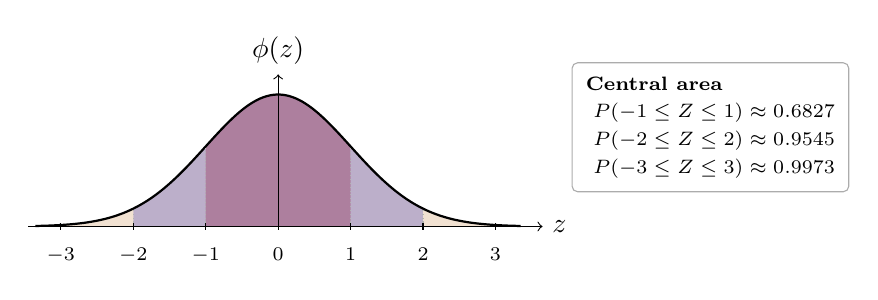
\begin{tikzpicture}[
    x=0.92cm,
    y=4.2cm,
    declare function={ gauss(\x) = exp(-0.5*(\x)^2)/(sqrt(2*pi)); }
]
  \fill[orange!70!black, opacity=0.18]
    (-3,0) -- plot[domain=-3:3, samples=100] (\x,{gauss(\x)}) -- (3,0) -- cycle;
  \fill[blue!70!black, opacity=0.22]
    (-2,0) -- plot[domain=-2:2, samples=100] (\x,{gauss(\x)}) -- (2,0) -- cycle;
  \fill[purple!70!black, opacity=0.28]
    (-1,0) -- plot[domain=-1:1, samples=100] (\x,{gauss(\x)}) -- (1,0) -- cycle;

  \draw[->] (-3.45,0) -- (3.65,0) node[right] {$z$};
  \draw[->] (0,0) -- (0,0.46) node[above] {$\phi(z)$};
  \draw[thick, domain=-3.35:3.35, samples=150] plot (\x,{gauss(\x)});

  \foreach \x in {-3,-2,-1,1,2,3}{
    \draw[densely dotted, gray!60] (\x,0) -- (\x,{gauss(\x)});
  }
  \foreach \x/\lab in {
    -3/{$-3$}, -2/{$-2$}, -1/{$-1$},
     0/{$0$},
     1/{$1$}, 2/{$2$}, 3/{$3$}
  }{
    \draw (\x,0.01) -- (\x,-0.01)
      node[below=3pt, font=\scriptsize] {\lab};
  }

  \node[
    anchor=west,
    align=left,
    font=\scriptsize,
    fill=white,
    draw=gray!65,
    rounded corners=2pt,
    inner sep=5pt
  ] at (4.05,0.30) {
    \textbf{Central area}\\[2pt]
    \textcolor{purple!70!black}{$\blacksquare$}\ $P(-1\le Z\le1)\approx0.6827$\\[2pt]
    \textcolor{blue!70!black}{$\blacksquare$}\ $P(-2\le Z\le2)\approx0.9545$\\[2pt]
    \textcolor{orange!70!black}{$\blacksquare$}\ $P(-3\le Z\le3)\approx0.9973$
  };
\end{tikzpicture}
\end{center}
\noindent\textit{Figure: the standard normal curve with the central one-, two-, and three-standard-deviation regions shaded.}
